\documentclass[a4paper, 11pt]{article}
 
\usepackage[utf8]{inputenc}
\usepackage{graphicx}
\usepackage[frenchb]{babel}
\usepackage{makecell}
\usepackage{listings}
\usepackage[dvipsnames]{xcolor}
\usepackage{graphicx}

\lstset{language=C,
	 	basicstyle=\ttfamily,
		keywordstyle=\ttfamily\textcolor{RubineRed},
		identifierstyle=,columns=fullflexible,
		commentstyle=\textcolor{OliveGreen},
		showstringspaces=false, breaklines=true,tabsize=4}

\usepackage{graphicx} %pour les images

\usepackage{xcolor}

\setcounter{tocdepth}{3}
\definecolor{Zgris}{rgb}{0.87,0.85,0.85}

\newsavebox{\BBbox}
\newenvironment{DDbox}[1]{
\begin{lrbox}{\BBbox}\begin{minipage}{\linewidth}}
{\end{minipage}\end{lrbox}\noindent\colorbox{Zgris}{\usebox{\BBbox}} \\
[.5cm]}

\begin{document}
 
\title{PROJET: Sodelisation et Verification du Comportement de Vehicules Aautomatiques sur un Pont a Voie Unique}
\author{Ilyas Toumlilt\\Maxime Bittan\\Redha Gouicem}
\date{05/12/2015}
 
\maketitle

\section{Question 1.1}
Les interfaces entre les différents composants sont les suivantes :\\
\begin{itemize}
\item Entre CTRLP et VAA : askA (transition) et exitVAA (transition)\\
\item Entre CTRLP et VAB : askB (transition) et exitVAB (transition)\\
\item Entre P et VAA : goToBridge (place) et exitBridge (place)\\
\item Entre P et VAB : goToBridge (place) et exitBridge (place)\\
\end{itemize}

\section{Question 1.2}
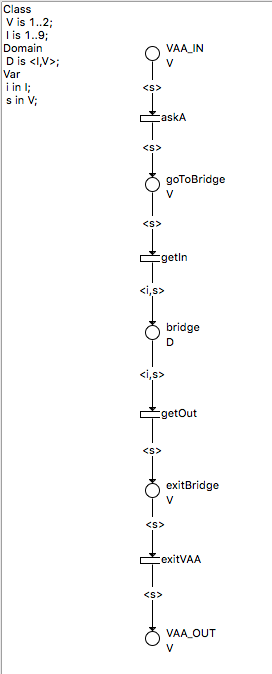
\includegraphics[scale=0.35]{VAA.png}


\section{Question 1.3}
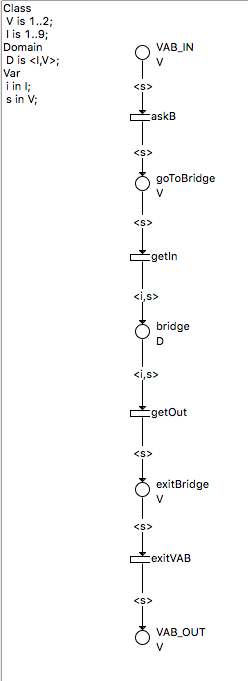
\includegraphics[scale=0.35]{VAB.png}

\section{Question 1.4}
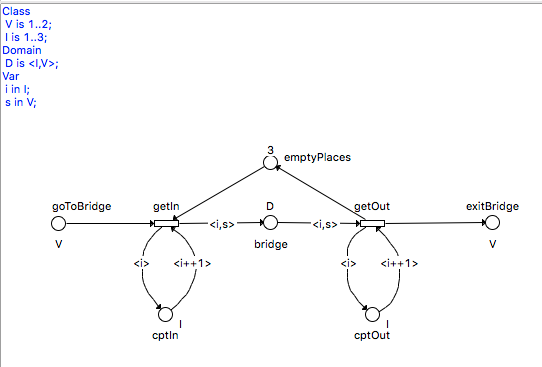
\includegraphics[scale=0.35]{P.png}
Afin de verifier le comportement de ce composant, nous avons verifié les propriétés suivantes :
\begin{itemize}
\item Le pont ne contient jamais plus de N éléments. Voir fichier pp1.txt.
\item A une position donné du pont, il n'y a qu'un seul vehicule. Voir fichier pp2.txt.
\end{itemize}

\section{Question 1.5}
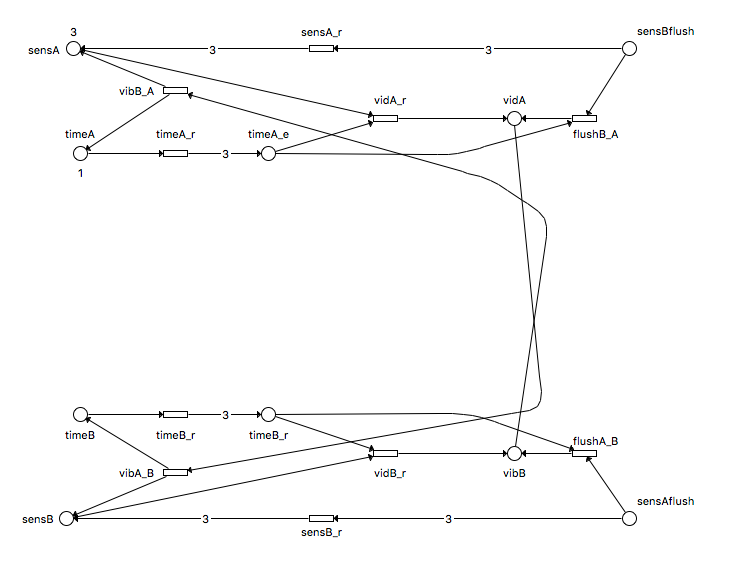
\includegraphics[scale=0.35]{CTRLP.png}

\section{Question 1.6}
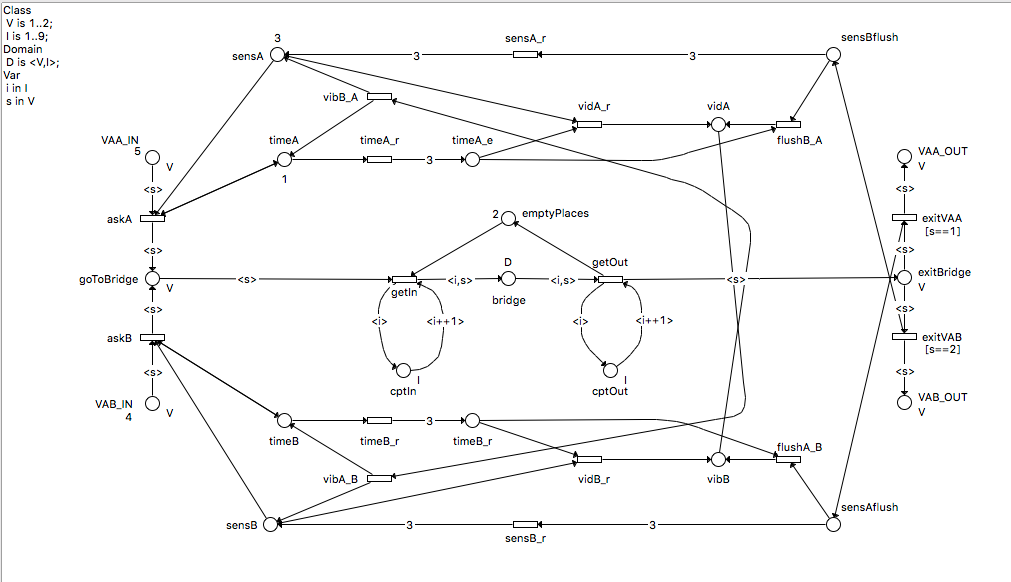
\includegraphics[scale=0.35]{bridge.png}

\section{Question 1.7}
p1 pour VAA : implies(card(VAA\_IN)=1, AF(card(VAA\_OUT)=1))
p1 pour VAB : implies(card(VAB\_IN)=1, AF(card(VAB\_OUT)=1))
p2 : G((card(emptyPlaces)+card(bridge))=2)

\end{document}
